\documentclass{article}

\usepackage{times}
\usepackage{geometry}
\geometry{a4paper,left=0.6cm,right=0.7cm,top=1cm,bottom=1cm,columnsep=0.8cm}

\usepackage{fontawesome}
\usepackage[hidelinks]{hyperref}
\usepackage{multicol,paracol,tikz,hyphsubst,moresize,hyphenat,adjustbox,tabularx,xcolor,enumitem}
\usepackage{ragged2e}
\newcolumntype{Y}{>{\RaggedRight\arraybackslash}X}
\setlist[itemize]{itemsep=1pt,leftmargin=*,topsep=-10pt}

\definecolor{maincolor}{HTML}{ffffff}
\definecolor{seccolor}{HTML}{0b1f3b}
\definecolor{gray}{HTML}{8c94a9}
\definecolor{sidetext}{HTML}{59cee5}
\definecolor{Green}{HTML}{2caf00}
\definecolor{lightgray}{HTML}{D3D3D3}

% --- bande latérale bleue
\usepackage{eso-pic}
\AddToShipoutPictureBG{%
  \begin{tikzpicture}[remember picture,overlay]
    \fill[seccolor] (0.7\paperwidth,0) rectangle (\paperwidth,\paperheight);
    \fill[maincolor] (0,0) rectangle (0.7\paperwidth,\paperheight);
  \end{tikzpicture}%
}

\setlength{\parindent}{0pt}
\newcommand{\cvsection}[1]{%
  \par\bigskip                % espace avant le titre
  {\bfseries\Large #1}\par
  \noindent\rule{\linewidth}{0.8pt}\par
  \medskip                    % espace après la ligne
}

\newcommand*{\ClipSep}{0.4cm}

% ------------------------------------------------------------------
\begin{document}\pagestyle{empty}
\columnratio{0.7}\begin{paracol}{2}

% --------- colonne gauche -----------------------------------------
\begin{minipage}{0.7\linewidth}
{\LARGE\textbf{Judikael Mourouvin}}

\bigskip
{\large\textbf{Technicien informatique \& marketing digital}}
\end{minipage}\hfill
\begin{minipage}{0.18\linewidth}
\begin{tikzpicture}
\node[inner sep=0pt]{ 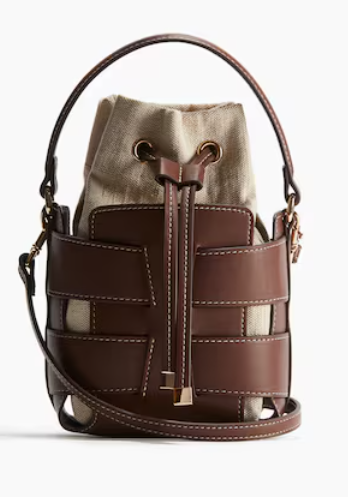
\includegraphics[width=\linewidth]{a8258724c58f4c89b84416df2d215d9c.png} };
\draw[white,rounded corners=\ClipSep,line width=\ClipSep]
      (current bounding box.north west) --
      (current bounding box.north east) --
      (current bounding box.south east) --
      (current bounding box.south west) -- cycle;
\end{tikzpicture}
\end{minipage}

\cvsection{Profil}
Passionné par l’informatique et le marketing digital, je possède une solide expérience en assistance technique et en gestion de projets numériques. Mon année d’alternance à la DSI de la Mairie du Gosier m’a permis de renforcer mes compétences en support utilisateur et en déploiement de solutions adaptées. Rigoureux, polyvalent et orienté résultat, je maîtrise aussi bien la configuration des réseaux que les leviers de communication en ligne. Je souhaite désormais m’investir à temps plein pour accompagner vos équipes et contribuer à la réussite de vos initiatives digitales.

\cvsection{EXPÉRIENCE}

\colorbox{maincolor}{%
  \begin{minipage}{\linewidth}
    \textbf{Alternant en Marketing Digital} \\ Mairie du Gosier - DSI \\ 2023-2024
    \begin{itemize}
      \item Géré des projets numériques municipaux et assuré leur déploiement dans les délais. \item Analysé les besoins des usagers et implémenté des solutions digitales adaptées. \item Formé et assisté les agents, renforçant l’adoption des outils et la satisfaction utilisateur.
    \end{itemize}
  \end{minipage}}

\vspace{3mm}


\colorbox{maincolor}{%
  \begin{minipage}{\linewidth}
    \textbf{Animateur de la zone informatique} \\ Pôle Emploi, Gosier \\ 2022-2023
    \begin{itemize}
      \item Fournit un support quotidien aux demandeurs et conseillers, réduisant les temps d’attente. \item Configuré et entretenu le parc informatique pour garantir la disponibilité des postes. \item Diagnostiqué et résolu les pannes, améliorant la continuité de service.
    \end{itemize}
  \end{minipage}}

\vspace{3mm}


\colorbox{maincolor}{%
  \begin{minipage}{\linewidth}
    \textbf{Stagiaire Informaticien} \\ Numerika, Baie-Mahault \\ 2020-2021
    \begin{itemize}
      \item Configuré et maintenu les équipements informatiques afin d’assurer leur bon fonctionnement. \item Apporté un support de proximité, facilitant la résolution rapide d’incidents pour les utilisateurs.
    \end{itemize}
  \end{minipage}}

\cvsection{FORMATION}

    \begin{tabularx}{\linewidth}{@{}c >{\RaggedRight\arraybackslash}X@{}}
    \textcolor{sidetext}{\faGraduationCap} &
    \textbf{Bachelor Marketing Digital} \\
    & CFA IUTS \\
    & \textit{2023-2024} \\
    \end{tabularx}
    \begin{itemize}[leftmargin=*]
  \item Approfondissement des stratégies de communication digitale et de SEO.
  \item Projets pratiques en gestion de campagnes et analyse de données.
  \item Utilisation des outils de marketing automation et des réseaux sociaux.
\end{itemize}
\vspace{3mm}

    \begin{tabularx}{\linewidth}{@{}c >{\RaggedRight\arraybackslash}X@{}}
    \textcolor{sidetext}{\faGraduationCap} &
    \textbf{BTS Système Numérique option Informatique et Réseaux} \\
    & Lycée de Chevalier Saint Georges, Abymes \\
    & \textit{2019-2021} \\
    \end{tabularx}
    \begin{itemize}[leftmargin=*]
  \item Étude des architectures réseau et administration de systèmes.
  \item Travaux pratiques en maintenance hardware et logiciels embarqués.
  \item Initiation à la cybersécurité et à la programmation appliquée.
\end{itemize}

% --------- colonne droite (bleue) ---------------------------------
\switchcolumn\color{white}\hspace*{0.4cm}\begin{minipage}{0.88\linewidth}

\cvsection{CONTACT}
\begin{tabular}{@{}c l}
  \faPhone & \href{tel:+590 0690 91 14 48}{+590 0690 91 14 48} \\[2pt]
  \faEnvelope & \href{mailto:jkmou971@gmail.com}{jkmou971@gmail.com} \\[2pt]
  \faMapMarker & Route de Cocoyer\,97190 Gosier \\[2pt]
  \faLinkedin & \href{}{}
\end{tabular}

\cvsection{COMPÉTENCES}

\begin{itemize}[leftmargin=*]
\item Administration
\item Réseaux
\item Assistance
\item Maintenance
\item Diagnostic
\item Configuration
\item Marketing\end{itemize}
\par\bigskip 

\cvsection{LANGUES}
\begin{itemize}[leftmargin=*]
\item Anglais - \textcolor{gray}{}
\item Espagnol - \textcolor{gray}{}\end{itemize}
\par\bigskip 
\cvsection{INTÉRÊTS}
\begin{itemize}[leftmargin=*]
\item Lectur
\item Sports
\item Musique
\item Voyage
\end{itemize}

\end{minipage}
\end{paracol}
\end{document}
